\documentclass[12pt,a4paper]{article}
\usepackage[utf8]{vietnam}
\usepackage{amsmath,amssymb}
\usepackage{tabularx}
\usepackage{tikz}
\usetikzlibrary{calc,arrows.meta}
\usepackage{xcolor}
\usepackage{enumitem}
\usepackage{fancyhdr}
\usepackage[top=1.2cm, bottom=1.2cm, left=1.5cm, right=1.5cm]{geometry}
\usepackage[loigiai]{ex_test}
\SAOPTN{widthSA=2.6,heightSA=0.62}

\setlength{\headheight}{15pt}
\setlength{\parskip}{0pt}

\pagestyle{fancy}
\fancyhf{}
\rhead{\textit{Lời giải chi tiết -- Đề số 7}}
\lhead{\textit{Bộ đề ôn tập Giữa học kì I -- Toán 7}}
\cfoot{\thepage}

\begin{document}

\begin{center}
\textbf{\Large HƯỚNG DẪN CHẤM VÀ LỜI GIẢI CHI TIẾT}\\
\vspace{1.5mm}
\textbf{\large MÔN: TOÁN 7 -- ĐỀ SỐ 7}
\end{center}
\vspace{2mm}

\noindent\textbf{\large PHẦN I. CÂU TRẮC NGHIỆM NHIỀU PHƯƠNG ÁN LỰA CHỌN}

\vspace{1mm}
\begin{ex}
Trong các số sau, số nào KHÔNG phải là số hữu tỉ?
\choice
{$-\dfrac{5}{6}$}
{$1\dfrac{2}{3}$}
{\True $\dfrac{7}{0}$}
{$-0{,}85$}
\loigiai{
Số hữu tỉ là số viết được dưới dạng $\dfrac{a}{b}$ với $a, b \in \mathbb{Z}, b \neq 0$. Phân số $\dfrac{7}{0}$ có mẫu số bằng $0$ nên không phải là số hữu tỉ.
}
\end{ex}

\begin{ex}
Số đối của số hữu tỉ $-\dfrac{3}{8}$ là:
\choice
{\True $\dfrac{3}{8}$}
{$\dfrac{8}{3}$}
{$-\dfrac{3}{8}$}
{$-\dfrac{8}{3}$}
\loigiai{
Số đối của số hữu tỉ $x$ là $-x$. Do đó số đối của $-\dfrac{3}{8}$ là $-\left(-\dfrac{3}{8}\right) = \dfrac{3}{8}$.
}
\end{ex}

\begin{ex}
Kết quả của phép tính $5^4 \cdot 5^7$ viết dưới dạng một lũy thừa là:
\choice
{$5^{28}$}
{\True $5^{11}$}
{$25^{11}$}
{$5^3$}
\loigiai{
Áp dụng công thức nhân hai lũy thừa cùng cơ số: $a^m \cdot a^n = a^{m+n}$:
\[ 5^4 \cdot 5^7 = 5^{4+7} = 5^{11}. \]
}
\end{ex}

\begin{ex}
Bỏ dấu ngoặc của biểu thức $A = -(m - n + p - q)$ ta được:
\choice
{$-m - n + p - q$}
{\True $-m + n - p + q$}
{$-m + n + p + q$}
{$-m - n - p - q$}
\loigiai{
Khi bỏ dấu ngoặc có dấu trừ đằng trước, ta đổi dấu tất cả các số hạng bên trong: $-(m - n + p - q) = -m + n - p + q$.
}
\end{ex}

\begin{ex}
So sánh hai số hữu tỉ $-0{,}6$ và $-\dfrac{3}{4}$, khẳng định nào sau đây đúng?
\choice
{$-0{,}6 < -\dfrac{3}{4}$}
{$-0{,}6 = -\dfrac{3}{4}$}
{\True $-0{,}6 > -\dfrac{3}{4}$}
{$-0{,}6 \le -\dfrac{3}{4}$}
\loigiai{
Ta có $-\dfrac{3}{4} = -0{,}75$. Vì $-0{,}6 > -0{,}75$ nên $-0{,}6 > -\dfrac{3}{4}$.
}
\end{ex}

\begin{ex}
Căn bậc hai số học của $81$ là:
\choice
{\True $9$}
{$-9$}
{$9$ và $-9$}
{$81$}
\loigiai{
Căn bậc hai số học của số $a \ge 0$ là số không âm $\sqrt{a}$. Do $9 > 0$ và $9^2 = 81$ nên căn bậc hai số học của $81$ là $9$.
}
\end{ex}

\begin{ex}
Trong các số sau, số nào là số vô tỉ?
\choice
{$\sqrt{25}$}
{$1{,}(3)$}
{\True $\sqrt{5}$}
{$-3{,}14$}
\loigiai{
Ta có $\sqrt{25} = 5$ (số hữu tỉ), $1{,}(3) = \dfrac{4}{3}$ (số hữu tỉ), $-3{,}14 = -\dfrac{157}{50}$ (số hữu tỉ). Số $\sqrt{5} \approx 2{,}236\dots$ là số thập phân vô hạn không tuần hoàn nên là số vô tỉ.
}
\end{ex}

\begin{ex}
Một hình lăng trụ đứng có diện tích đáy $S = 15\text{ cm}^2$ và chiều cao $h = 8\text{ cm}$. Thể tích $V$ của hình lăng trụ đứng đó là:
\choice
{\True $120\text{ cm}^3$}
{$60\text{ cm}^3$}
{$40\text{ cm}^3$}
{$23\text{ cm}^3$}
\loigiai{
Thể tích hình lăng trụ đứng: $V = S \cdot h = 15 \cdot 8 = 120\text{ cm}^3$.
}
\end{ex}

\begin{ex}
Trong định lí: ''Nếu hai đường thẳng phân biệt cùng vuông góc với một đường thẳng thứ ba thì chúng song song với nhau'', phần kết luận là:
\choice
{Hai đường thẳng phân biệt cùng vuông góc với đường thẳng thứ ba}
{\True Chúng song song với nhau}
{Hai đường thẳng vuông góc với nhau}
{Đường thẳng thứ ba vuông góc với hai đường thẳng}
\loigiai{
Trong định lí có dạng ''Nếu $A$ thì $B$'', phần sau từ ''thì'' là kết luận: ''Chúng song song với nhau''.
}
\end{ex}

\begin{ex}
Cho điểm $M$ nằm ngoài đường thẳng $d$. Số đường thẳng đi qua $M$ và song song với $d$ là:
\choice
{$0$}
{\True $1$}
{$2$}
{Vô số}
\loigiai{
Theo tiên đề Euclid, qua một điểm nằm ngoài một đường thẳng chỉ có duy nhất một đường thẳng song song với đường thẳng đó.
}
\end{ex}

\begin{ex}
Cho $a \parallel b$, đường thẳng $c$ cắt cả $a$ và $b$. Biết một góc trong cùng phía có số đo bằng $70^\circ$, số đo của góc trong cùng phía còn lại là:
\choice
{$70^\circ$}
{\True $110^\circ$}
{$180^\circ$}
{$20^\circ$}
\loigiai{
Vì $a \parallel b$ nên hai góc trong cùng phía bù nhau, do đó số đo của góc trong cùng phía còn lại là $180^\circ - 70^\circ = 110^\circ$.
}
\end{ex}

\begin{ex}
Cho $\Delta MNP = \Delta DEF$. Khẳng định nào sau đây là đúng?
\choice
{$MN = DF$}
{$MP = DE$}
{\True $NP = EF$}
{$\widehat{M} = \widehat{E}$}
\loigiai{
Vì $\Delta MNP = \Delta DEF$ nên các cạnh tương ứng bằng nhau: $MN = DE, NP = EF, MP = DF$. Do đó khẳng định C đúng.
}
\end{ex}


\setcounter{ex}{0}
\noindent\textbf{\large PHẦN II. CÂU TRẮC NGHIỆM ĐÚNG SAI}

\vspace{1mm}
\begin{ex}
Cho hai số hữu tỉ $x = -\dfrac{3}{5}$ và $y = \dfrac{2}{3}$. Xét tính đúng sai của các mệnh đề sau:
\choiceTF
{\True Số $x$ là số hữu tỉ âm, số $y$ là số hữu tỉ dương}
{\True Tổng $x + y$ có giá trị bằng $\dfrac{1}{15}$}
{\True Tích $x \cdot y$ có giá trị bằng $-\dfrac{2}{5}$}
{Số đối của $x$ nhỏ hơn số đối của $y$}
\loigiai{
\begin{itemize}[leftmargin=0.5cm, itemsep=1pt]
\item \textbf{a)} \textbf{Đúng}. Ta có $x = -\dfrac{3}{5} < 0$ nên $x$ là số hữu tỉ âm, $y = \dfrac{2}{3} > 0$ nên $y$ là số hữu tỉ dương.
\item \textbf{b)} \textbf{Đúng}. Ta có $x + y = -\dfrac{3}{5} + \dfrac{2}{3} = -\dfrac{9}{15} + \dfrac{10}{15} = \dfrac{1}{15}$.
\item \textbf{c)} \textbf{Đúng}. Ta có $x \cdot y = \left(-\dfrac{3}{5}\right) \cdot \dfrac{2}{3} = \dfrac{-3 \cdot 2}{5 \cdot 3} = -\dfrac{2}{5}$.
\item \textbf{d)} \textbf{Sai}. Số đối của $x$ là $-x = \dfrac{3}{5} = \dfrac{9}{15}$. Số đối của $y$ là $-y = -\dfrac{2}{3} = -\dfrac{10}{15}$. Vì $\dfrac{9}{15} > -\dfrac{10}{15}$ nên số đối của $x$ lớn hơn số đối của $y$.
\end{itemize}
}
\end{ex}

\begin{ex}
Cho hai đường thẳng $a$ và $b$ song song với nhau. Đường thẳng $c$ cắt đường thẳng $a$ tại điểm $A$ và cắt đường thẳng $b$ tại điểm $B$. Biết rằng trong bốn góc tạo thành tại đỉnh $A$, có một góc bằng $60^\circ$. Xét tính đúng sai của các mệnh đề sau:
\choiceTF
{\True Góc kề bù với góc $60^\circ$ tại đỉnh $A$ có số đo bằng $120^\circ$}
{Góc so le trong với góc $60^\circ$ tại đỉnh $B$ có số đo bằng $120^\circ$}
{\True Góc đồng vị với góc $60^\circ$ tại đỉnh $B$ có số đo bằng $60^\circ$}
{\True Hai góc trong cùng phía được tạo bởi đường thẳng $c$ cắt hai đường thẳng $a, b$ có tổng số đo bằng $180^\circ$}
\loigiai{
\begin{itemize}[leftmargin=0.5cm, itemsep=1pt]
\item \textbf{a)} \textbf{Đúng}. Hai góc kề bù có tổng số đo bằng $180^\circ$, do đó số đo góc kề bù là $180^\circ - 60^\circ = 120^\circ$.
\item \textbf{b)} \textbf{Sai}. Vì $a \parallel b$ nên hai góc so le trong có số đo bằng nhau, do đó góc so le trong với góc $60^\circ$ phải có số đo bằng $60^\circ$.
\item \textbf{c)} \textbf{Đúng}. Vì $a \parallel b$ nên hai góc đồng vị bằng nhau: số đo bằng $60^\circ$.
\item \textbf{d)} \textbf{Đúng}. Vì $a \parallel b$ nên hai góc trong cùng phía bù nhau (tổng số đo bằng $180^\circ$).
\end{itemize}
}
\end{ex}


\setcounter{ex}{0}
\noindent\textbf{\large PHẦN III. CÂU HỎI TRẢ LỜI NGẮN}

\vspace{1mm}
\begin{ex}
Tìm số hữu tỉ $x$, biết: $\left(x + \dfrac{1}{2}\right)^3 = -\dfrac{1}{27}$. \shortans{$x = -\dfrac{5}{6}$}
\loigiai{
Ta có $-\dfrac{1}{27} = \left(-\dfrac{1}{3}\right)^3$.
Suy ra $x + \dfrac{1}{2} = -\dfrac{1}{3} \implies x = -\dfrac{1}{3} - \dfrac{1}{2} = -\dfrac{5}{6}$.
}
\end{ex}

\begin{ex}
Tìm số thực $x$, biết: $|x - 0{,}5| + 0{,}75 = 2{,}25$. \shortans{$x = 2$ hoặc $x = -1$}
\loigiai{
Ta có $|x - 0{,}5| = 2{,}25 - 0{,}75 = 1{,}5$.
Xét hai trường hợp:
- Trường hợp 1: $x - 0{,}5 = 1{,}5 \implies x = 2$.
- Trường hợp 2: $x - 0{,}5 = -1{,}5 \implies x = -1$.
Vậy $x = 2$ hoặc $x = -1$.
}
\end{ex}


\setcounter{ex}{0}
\noindent\textbf{\large PHẦN IV. TỰ LUẬN}

\vspace{1mm}
\begin{ex}
Thực hiện phép tính (tính hợp lý nếu có):
\begin{enumerate}[label=\textbf{\alph*)}, leftmargin=0.8cm, itemsep=1pt]
\item $\dfrac{7}{6} - \dfrac{1}{6} + \dfrac{5}{8}$;
\item $-\dfrac{5}{13} \cdot \dfrac{2}{5} + \dfrac{5}{13} \cdot \left(-\dfrac{3}{5}\right)$;
\item $\left[\left(\dfrac{2}{3} - 0{,}25\right) + (-2)^2 \cdot \dfrac{3}{16}\right] - 1$.
\end{enumerate}
\loigiai{
\textbf{a)} \[ \dfrac{7}{6} - \dfrac{1}{6} + \dfrac{5}{8} = \left(\dfrac{7}{6} - \dfrac{1}{6}\right) + \dfrac{5}{8} = 1 + \dfrac{5}{8} = \dfrac{13}{8}. \]

\textbf{b)} \[ -\dfrac{5}{13} \cdot \dfrac{2}{5} + \dfrac{5}{13} \cdot \left(-\dfrac{3}{5}\right) = \dfrac{5}{13} \cdot \left(-\dfrac{2}{5} - \dfrac{3}{5}\right) = \dfrac{5}{13} \cdot (-1) = -\dfrac{5}{13}. \]

\textbf{c)} \[ \begin{aligned} \left[\left(\dfrac{2}{3} - \dfrac{1}{4}\right) + 4 \cdot \dfrac{3}{16}\right] - 1 &= \left[\left(\dfrac{8}{12} - \dfrac{3}{12}\right) + \dfrac{3}{4}\right] - 1 \\ &= \left[\dfrac{5}{12} + \dfrac{9}{12}\right] - 1 = \dfrac{14}{12} - 1 = \dfrac{7}{6} - 1 = \dfrac{1}{6}. \end{aligned} \]

}
\end{ex}
\vspace{1.5mm}

\begin{ex}
Tìm $x$:
\begin{enumerate}[label=\textbf{\alph*)}, leftmargin=0.8cm, itemsep=1pt]
\item $x - \dfrac{1}{9} = -\dfrac{5}{6}$;
\item $-\dfrac{1}{5} + \dfrac{6}{5} : x = (-2)^2$.
\end{enumerate}
\loigiai{
\textbf{a)} \[ x = -\dfrac{5}{6} + \dfrac{1}{9} = -\dfrac{15}{18} + \dfrac{2}{18} = -\dfrac{13}{18}. \]

\textbf{b)} \[ \begin{aligned} -\dfrac{1}{5} + \dfrac{6}{5} : x &= 4 \\ \dfrac{6}{5} : x &= 4 - \left(-\dfrac{1}{5}\right) = \dfrac{21}{5} \\ x &= \dfrac{6}{5} : \dfrac{21}{5} = \dfrac{6}{5} \cdot \dfrac{5}{21} = \dfrac{2}{7}. \end{aligned} \]

}
\end{ex}
\vspace{1.5mm}

\begin{ex}
\immini{
Cho hình vẽ, biết $\widehat{yOz} = 50^\circ$.
\begin{enumerate}[label=\textbf{\alph*)}, leftmargin=0.8cm, itemsep=1pt]
\item Kể tên các cặp góc kề bù trong hình vẽ.
\item Kẻ $Ot$ là tia phân giác của $\widehat{xOz}$. Tính số đo $\widehat{xOz}$ và $\widehat{xOt}$.
\end{enumerate}
}{
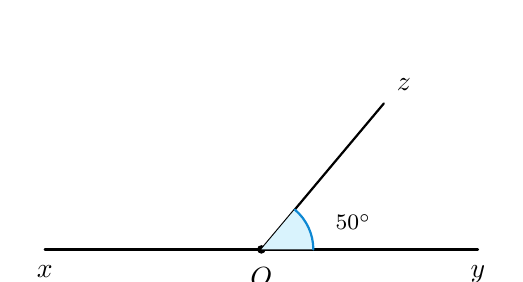
\begin{tikzpicture}[scale=1.1, line cap=round, line join=round]
    \coordinate (O) at (0, 0);
    \coordinate (X) at (-2.5, 0);
    \coordinate (Y) at (2.5, 0);
    \coordinate (Z) at (50:2.2);

    \draw[thick] (X) node[below=2pt] {$x$} -- (Y) node[below=2pt] {$y$};
    \draw[thick] (O) -- (Z) node[above right=1pt] {$z$};

    \filldraw[black] (O) circle (1.2pt) node[below=3pt] {$O$};

    \fill[cyan!15] (O) -- (0:0.6) arc (0:50:0.6) -- cycle;
    \draw[cyan!70!blue, thick] (0:0.6) arc (0:50:0.6);
    \node[font=\footnotesize, right=2pt] at (25:0.75) {$50^\circ$};
\end{tikzpicture}
}
\loigiai{
\textbf{a)} Cặp góc kề bù trong hình là $\widehat{xOz}$ và $\widehat{yOz}$.

\textbf{b)} Vì $\widehat{xOz}$ và $\widehat{yOz}$ là hai góc kề bù nên:
\[ \widehat{xOz} + \widehat{yOz} = 180^\circ \implies \widehat{xOz} = 180^\circ - 50^\circ = 130^\circ. \]
Vì $Ot$ là tia phân giác của $\widehat{xOz}$ nên:
\[ \widehat{xOt} = \dfrac{\widehat{xOz}}{2} = \dfrac{130^\circ}{2} = 65^\circ. \]

}
\end{ex}
\vspace{1.5mm}

\begin{ex}
Tìm số hữu tỉ $x$ sao cho:
\[ \dfrac{x + 1}{2023} + \dfrac{x + 2}{2022} = \dfrac{x + 3}{2021} + \dfrac{x + 4}{2020}. \]
\loigiai{
Cộng thêm $2$ vào cả hai vế của phương trình:
\[ \left(\dfrac{x + 1}{2023} + 1\right) + \left(\dfrac{x + 2}{2022} + 1\right) = \left(\dfrac{x + 3}{2021} + 1\right) + \left(\dfrac{x + 4}{2020} + 1\right) \]
\[ \iff \dfrac{x + 2024}{2023} + \dfrac{x + 2024}{2022} = \dfrac{x + 2024}{2021} + \dfrac{x + 2024}{2020} \]
\[ \iff (x + 2024) \left(\dfrac{1}{2023} + \dfrac{1}{2022} - \dfrac{1}{2021} - \dfrac{1}{2020}\right) = 0. \]
Vì $2023 > 2021 \implies \dfrac{1}{2023} < \dfrac{1}{2021}$ và $2022 > 2020 \implies \dfrac{1}{2022} < \dfrac{1}{2020}$ nên:
\[ \dfrac{1}{2023} + \dfrac{1}{2022} - \dfrac{1}{2021} - \dfrac{1}{2020} \neq 0. \]
Do đó $x + 2024 = 0 \iff x = -2024$.
Vậy $x = -2024$.
}
\end{ex}
\vspace{1.5mm}


\begin{center}
\rule{4cm}{0.4pt}\\
\textit{--- HẾT ---}
\end{center}
\end{document}
